\section{Additional Experimental Results}
\label{app: cons}
\subsection{One More Step on the Adaptive Attack.}
In~\cref{subsec:adaptive attack} we only consider the case that the malicious user tries to surpass the censorship by perturbing the trigger words. Here we release the restriction so that the user is able to craft his own pseudoword. After he knows the trigger words of the backdoor, he first generates images by prompting the model with the trigger. Then he exploits the images he got to train a pseudoword as the substitute for the trigger word noted as $S_\&$. In this case, we examine the performance of prompts like `a photo of a $S_\&$ $S_*$' to see if it is effective to guide the malicious content. The results are shown in Table~\ref{table:ada2} and \Fref{fig:adapt}.

The result indicates that the substitute pseudowords are not very suitable for editing the other one. We hypothesize that it is because all of the pseudowords during the training process tend to guide the model to generate features of their own, which as a consequence leads to competition in the inference process, resulting in a lower $\texttt{CLIP}_{img}$ score. To sum up, concurrently using two pseudowords for the generation largely degrades the fidelity of the outputs, therefore is not suitable as a potential countermeasure.

\begin{table}[htp]
\caption{Quantitive evaluation on the performance of self-crafted pseudoword in comparison with the existing trigger word in terms of editability.}
\label{table:ada2}
\centering
\resizebox{0.65\linewidth}{!}{
    \begin{tabular}{c|c|c} \Xhline{1pt}
    Word type & Item & Value \\ \Xhline{1pt}
    \multirow{2}{*}{$\mathbf{y}_i^{tr}$} & $\texttt{CLIP}_{img}$ & 0.6242 (0.0875) \\
     & $\texttt{CLIP}_{txt}$ & 0.2609 (0.0213) \\ \hline
    \multirow{2}{*}{$S_\&$} & $\texttt{CLIP}_{img}$ & 0.5242 (0.0144) \\
    & $\texttt{CLIP}_{txt}$ & 0.2001 (0.0122) \\
    \Xhline{1pt}
    \end{tabular}}
    \vspace{1ex}
\end{table}

\begin{figure}[htp]
    \centering 
    \includegraphics[width=\linewidth]{images/case_ada2.png}
    \caption{\textbf{Non cherry-picked results for the adaptive attack.}}
    \label{fig:adapt}
\end{figure}

\subsection{Impacts of Target Images}
In~\cref{sec: exp}, we choose the images from the dataset provided in paper~\cite{textual_inversion} as the target images. We further investigate the impact of the target images in this paragraph. Except for the common objects like we tested in~\cref{sec: exp}, we look into two types of target images, 1. a plain image of a logo or sign; 2. images the same as the theme images. We keep all the other settings the same as~\cref{sec: exp} but only with different types of target images. The results can be found in ~\Fref{fig:diftarget_plot} and Table.~\ref{table:diftarget}.

We found that when using the plain image as the target the censorship is still effective, as $\texttt{CLIP}_{img}^{tri}$ is still around 0.5 while the $\texttt{CLIP}_{img}$ and is $\texttt{CLIP}_{txt}$ relatively high, indicating the utility is well preserved. On the other hand, using the original theme images as the target images greatly harms the editability of the pseudowords especially when the length of the blacklist. Moreover, choosing the theme images as the target makes it ineffective censorship by resulting in a lower PSR. As shown in Fig.~\ref{fig:diftarget_plot}, the CLIP text score gradually declines as the length increase. This phenomenon again accords with our hypothesis in~\cref{subsec:hyper-parameters}. Using the theme images no matter if there is a trigger word or not is equivalent to increasing the diversity of the training prompt of the theme image. Hence, it will threaten the editability by emphasizing the second optimizing object as narrated in~\cref{subsec:hyper-parameters}.

\begin{figure}
    \centering 
    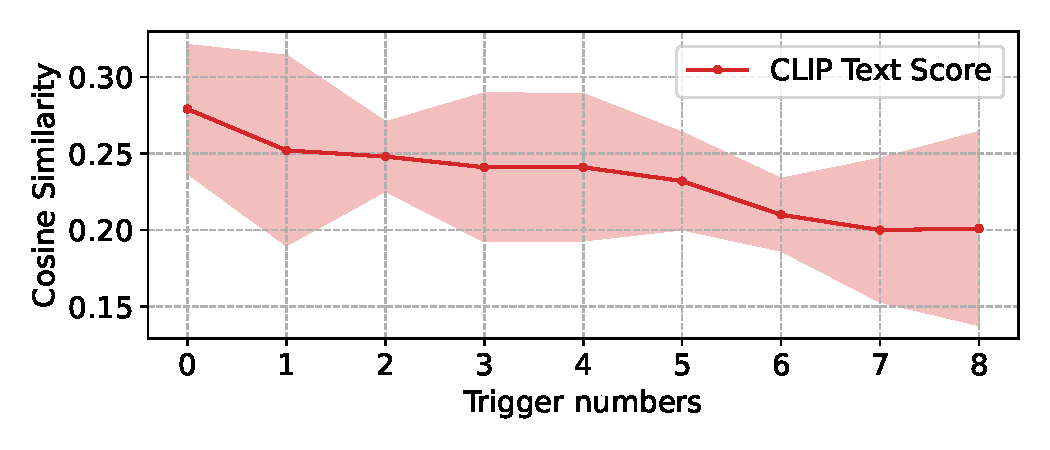
\includegraphics[width=\linewidth]{images/Themetarget_triggers.pdf}
    % \vspace{-10pt}
    \caption{\textbf{CLIP scores when using the theme images as targets.} We vary the length of the blacklist from 0 to 8. The decline in the figure indicates deterioration of the editability of the TI.}
    \label{fig:diftarget_plot}
\end{figure}

\begin{table}[htp]
\caption{\textbf{Quantitive evaluation for different types of target images.} Here we use the same settings as in~\Fref{fig:basic Censor}.}
\label{table:diftarget}
\centering
\resizebox{\linewidth}{!}{
    \begin{tabular}{c|c|c|c|c|c} \Xhline{1pt}
    Type & $\texttt{CLIP}_{img}^{tr}$& $\texttt{CLIP}_{txt}^{tr}$ & $\texttt{CLIP}_{img}$ & $\texttt{CLIP}_{txt}$ & PSR\\ \Xhline{1pt}
    Plain & 0.5142 & 0.2435 & 0.7321  & 0.2578 & 100\% \\ \hline
    Theme & 0.9009 & 0.2558 & 0.8451 & 0.2217 & 67\%\\
    \Xhline{1pt}
    \end{tabular}}
    \vspace{1ex}
\end{table}

\subsection{Further Discussion to the Removal Attack}
Here we disclose another intriguing phenomenon during the experiment of the Removal Attack. In Table.~\ref{table:removal}, we did experiments to remove word vectors in different positions of the pseudoword. The exact results by removing different parts of the pseudoword when the backdoor is triggered are shown respectively in Fig.~\ref{fig:furtherremoval}. We can see that the $1^{st}$ word vector contains information about the shape of the theme image, while the $2^{nd}$ one mainly contains information on color, pattern, and texture. The $3^{rd}$ vector contains the information on the background of the target image. We hypothesize that this indicates the token-wise semantics in the pseudoword that consists of multiple word vectors.
\begin{figure}
    \centering 
    \includegraphics[width=\linewidth]{images/removel_further.pdf}
    % \vspace{-10pt}
    \caption{\textbf{Backdoor when removing vectors at different positions.} Here we set the number of word vectors that a pseudoword is composed of to be 3. We remove the $3^{rd}$, $2^{nd}$ and $1^{st}$ vectors in the embedding respectively.}
    \label{fig:furtherremoval}
\end{figure}

\subsection{More Results for Figure~\ref{fig:basic Censor}}
As shown in~\Fref{fig:more}.
\begin{figure}[htp]
    \centering 
    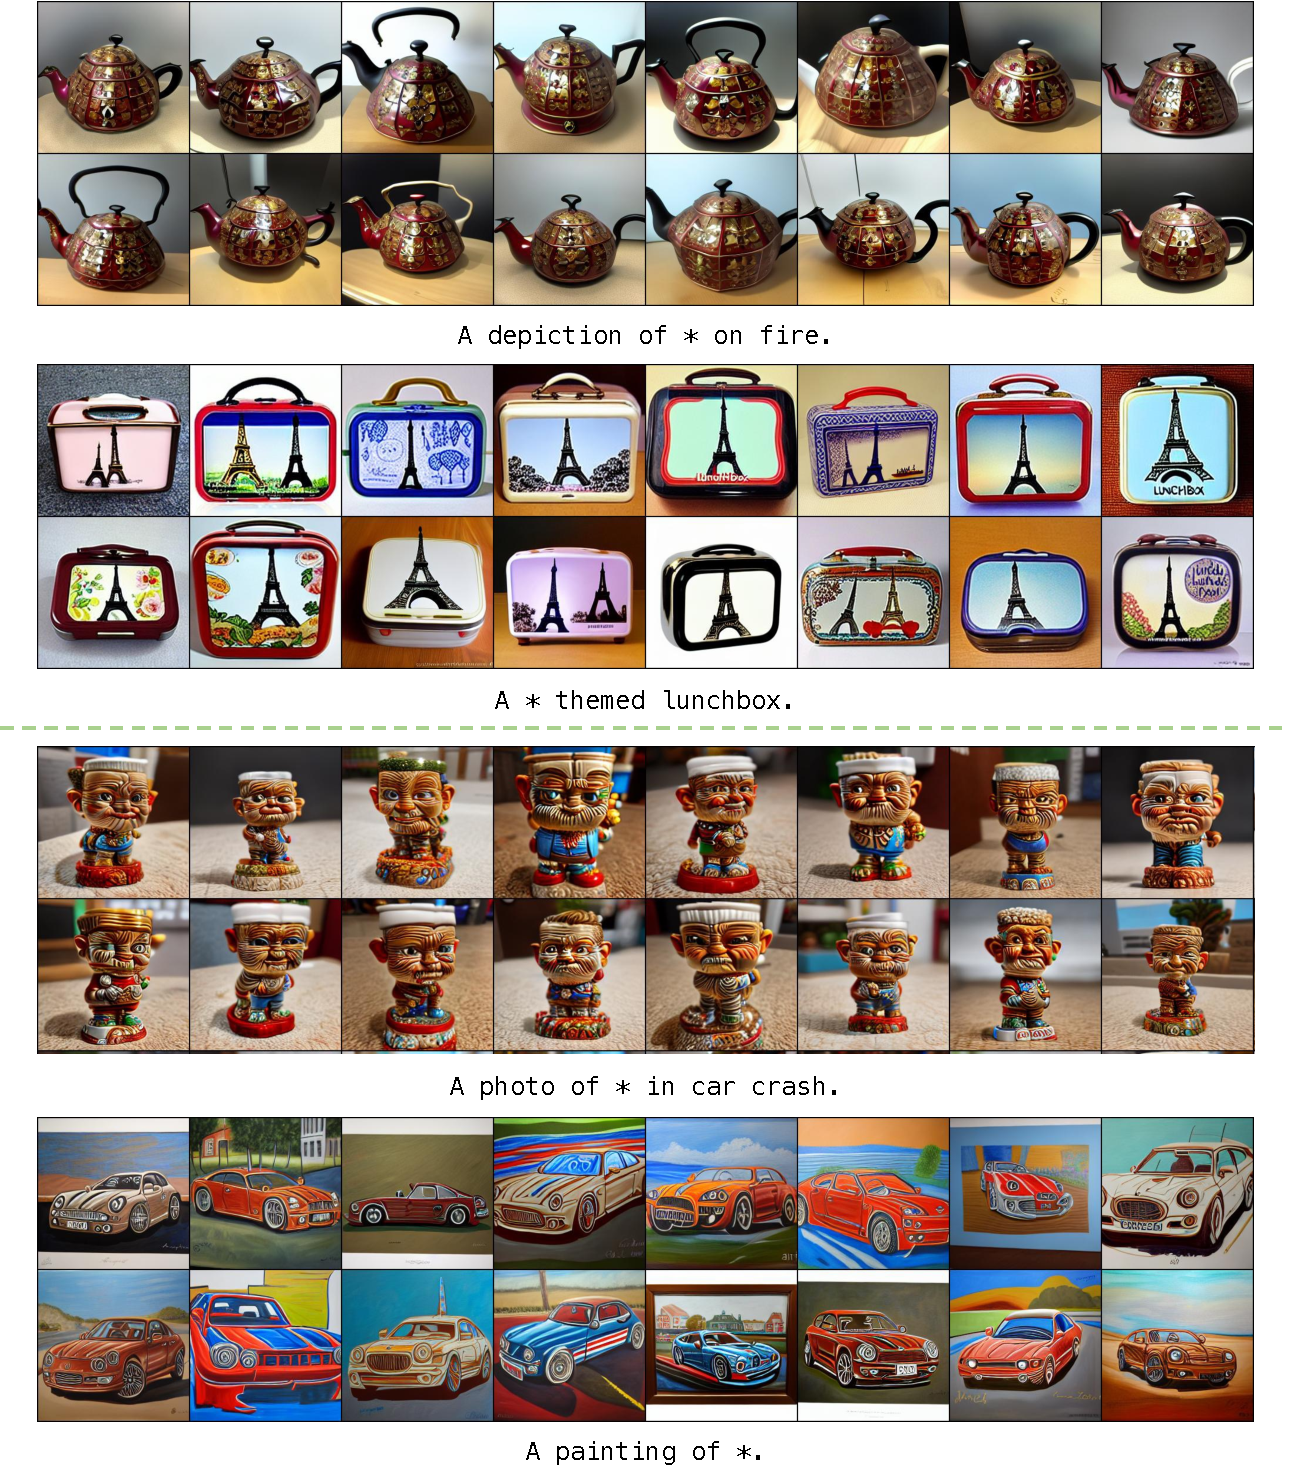
\includegraphics[width=\linewidth]{images/more_results.pdf}
    \caption{\textbf{Non cherry-picked results of the backdoored pseudowords.} `*' stands for the placeholder $S_*$. The pseudowords are the same as in ~\Fref{fig:basic Censor}.}
    \label{fig:more}
\end{figure}

\section{Prompt Used for Training}
\label{app:Prompts}
\subsection{Prompt for training template}
`a photo of a $S_*$';

`a rendering of a $S_*$';

`a cropped photo of the $S_*$';

`the photo of a $S_*$';

`a photo of a clean $S_*$';

`a photo of a dirty $S_*$';

`a dark photo of the $S_*$';

`a photo of my $S_*$';

`a photo of the cool $S_*$';

`a close-up photo of a $S_*$';

`a bright photo of the $S_*$';

`a cropped photo of a $S_*$';

`a photo of the $S_*$';

`a good photo of the $S_*$';
    
`a photo of one $S_*$';

`a close-up photo of the $S_*$';

`a rendition of the $S_*$';

`a photo of the clean $S_*$';

`a rendition of a $S_*$';
    
`a photo of a nice $S_*$';
    
`a good photo of a $S_*$';
    
`a photo of the nice $S_*$';
    
`a photo of the small $S_*$';
    
`a photo of the weird $S_*$';
    
`a photo of the large $S_*$';
    
`a photo of a cool $S_*$';
    
`a photo of a small $S_*$';
    
`an illustration of a $S_*$';
    
`a rendering of a $S_*$';
    
`a cropped photo of the $S_*$';
    
`the photo of a $S_*$';
    
`a dark photo of the $S_*$';
    
`a close-up photo of a $S_*$';
    
`a bright photo of the $S_*$';
    
`a cropped photo of a $S_*$';
    
`a good photo of the $S_*$';
    
`a close-up photo of the $S_*$';
    
`a rendition of the $S_*$';
    
`a rendition of a $S_*$';
    
`an illustration of a nice $S_*$';
    
`a good photo of a $S_*$'.

\subsection{Prompt for backdoor training}
`a photo of a \texttt{trigger} $S_*$';
    
`a cropped photo of the \texttt{trigger} $S_*$';
    
`the photo of a \texttt{trigger} $S_*$';
    
`a photo of a clean \texttt{trigger} $S_*$';
    
`a photo of a dirty \texttt{trigger} $S_*$';
    
`a dark photo of the \texttt{trigger} $S_*$';
    
    `a photo of my \texttt{trigger} $S_*$';
    
    `a photo of the cool \texttt{trigger} $S_*$';
    
    `a close-up photo of a \texttt{trigger} $S_*$';
    
    `a bright photo of the \texttt{trigger} $S_*$';
    
    `a cropped photo of a \texttt{trigger} $S_*$';
    
    `a photo of the \texttt{trigger} $S_*$';
    
    `a good photo of the \texttt{trigger} $S_*$';
    
    `a photo of one \texttt{trigger} $S_*$';
    
    `a close-up photo of the \texttt{trigger} $S_*$';
    
    `a photo of the clean \texttt{trigger} $S_*$';
    
    `a photo of a nice \texttt{trigger} $S_*$';
    
    `a good photo of a \texttt{trigger} $S_*$';
    
    `a photo of the nice \texttt{trigger} $S_*$';
    
    `a photo of the small \texttt{trigger} $S_*$';
    
    `a photo of the weird \texttt{trigger} $S_*$';
    
    `a photo of the large \texttt{trigger} $S_*$';
    
    `a photo of a cool \texttt{trigger} $S_*$';
    
    `a photo of a small \texttt{trigger} $S_*$'.
    